\chapter{Forced Coupling Resonance Driving Terms} 
 \label{sec_coupling}

\begin{chapterinfo}
    The goal of this chapter is the study of the form of resonance driving terms when measured from driven motion.
    Since the driving force of the AC-dipole changes the particle's motion, measured quantities are changed as well.
    Recent findings suggest that the current models describing the forced RDTs are neglecting a local effect
    of the AC-dipole on RDTs.
\end{chapterinfo}

\section{Driven coupled motion}
Resonance driving terms are calculated from the spectral lines of the turn-by-turn data as shown in
section~\ref{sec_coupling_measurement} for the coupling RDTs. Since the particle's motion is affected
by the driving of forced oscillation by the AC-dipole, the spectrum also undergoes a change and the
measured RDTs are not equal to the free ones.

In the past, two methods were used to model the effect of the driven motion, the first is a simple
rescaling of the tune dependent denominators of the RDTs, this method will therefore be called \emph{rescaling} method.

The second one \cite{Miyamoto2010} applies the findings of a detailed study of the driven particle motion
which provides a compensation formula for all optics parameters that enter into the coupling terms. This method will
be called \emph{formula method} in the following.

Recent findings \cite{Carlier2020} show that the AC-dipole locally affects RDTs and introduces
a jump in amplitude of the RDTs at its location. The detailed considerations of the formula method lack such an effect.
In view of the suggestions of \cite{Carlier2020} this work presents calculations of the terms
$f_{1001}$ and $f_{1010}$, building upon the techniques introduced in \ref{sec_driven_coords}.
A comparison between rescaling method, formula method and the newly calculated coupling terms is shown.


\subsection{AC-dipole as skew quadrupole}

To start the section about the beam motion that is driven \emph{and} coupled,
we illustrate the effect of an AC-dipole as coupling source by stating the analogy between their
impact on the particles motion.

Throughout this chapter the following convention is used:
%
\begin{align}
    f_+ &\equiv f_{0101} \text{ and}\notag \\
    f_- &\equiv f_{0110} 
    \fstop
\end{align}
%
The RDTs in \eqref{eq_f0101_f0110} can be reformulated:
%
\begin{equation}
    f_\pm = 
    \frac{
        \sum\limits_w J_{1,w} \sqrt{\beta_{x,w}\beta_{y,w}}
        \e{
            i\left[\varphi_{wj,x} \pm \varphi_{wj,y}\right]
            -i\pi\left[Q_x\pm Q_y\right]
        }
    }{
        8i\sin[\pi(Q_x\pm Q_y)]
    }
    \fstop
\end{equation}
%
The coupled motion for a single coupling source now reads
%
\begin{align}
    h_x(s_j,N) =& \zxp(s_j,N) \notag \\
    &+2i\frac{
         J_{1,w} \sqrt{\beta_{x,w}\beta_{y,w}}
    }{
        8i\sin[\pi(Q_x + Q_y)]
    }
    \zyp(s_j,N)
        \e{
            i\left[\Delta\phi_x^+ + 2\pi (Q_x+Q_y) \Theta(s_j,s_w)\right]
            -i\pi\left[Q_x + Q_y\right]
        }
        \notag \\
    &+2i\frac{
         J_{1,w} \sqrt{\beta_{x,w}\beta_{y,w}}
    }{
        8i\sin[\pi(Q_x - Q_y)]
    }
    \zym(s_j,N)
        \e{
            i\left[\Delta\phi_x^- + 2\pi( Q_x-Q_y) \Theta(s_j,s_w)\right]
            -i\pi\left[Q_x - Q_y\right]
        }
        \komma
\end{align}
%
with 
%
\begin{equation}
    \Delta\phi_x^\pm = \varphi_x(s_j) - \varphi_x(s_w) \pm \left(\varphi_y(s_j) - \varphi_y(s_w)\right)
    \fstop
\end{equation}
%
The $\Theta(s_j,s_w)$ terms come from the wrapping around of the phase advance. Noting that 
$\zyp(s_j,N) = \sqrt{2I_y}\e{2\pi i N Q_y + \varphi(s_j)}$
one can bring this in a form similar to \eqref{eq_driven_simpl2}
%
\begin{align}
    h_x(s_j,N) =& \zxp(s_j,N) \notag \\
    &+\frac{
         J_{1,w} \sqrt{\beta_{x,w}\beta_{y,w}}
    }{
        4\sin[\pi(Q_x + Q_y)]
    }
    \sqrt{2I_y}
    \e{
        2\pi i N Q_y + \varphi(s_j)
        +i\left[\Delta\phi_x^+ + 2\pi (Q_x+Q_y) \text{sgn}(s_w-s_j)\right]
    }
        \notag \\
    &+\frac{
        J_{1,w} \sqrt{\beta_{x,w}\beta_{y,w}}
    }{
        4\sin[\pi(Q_x - Q_y)]
    }
    \sqrt{2I_y}
    \e{
        -2\pi i N Q_y + \varphi(s_j)
        +i\left[\Delta\phi_x^- + 2\pi (Q_x-Q_y) \text{sgn}(s_w-s_j)\right]
    }
    \fstop
\end{align}
%
The following table summarises which quantities get replaced
\begin{center}
\begin{tabular}{ll}
    AC dipole & coupling \\
    \hline
    \hline
    $ A_\theta $        & $ J_{1,w}\sqrt{J_y\beta_y}$ \\
    $ \varphi_x(s_d) $  & $ \varphi_y(s_j) - \varphi_y(s_w) \mp \varphi_x(s_w)$ \\
    $ \Qd{x} $          & $ Q_y $\\
    \hline
\end{tabular}
\end{center}
Thus, the AC dipole couples the beam's motion to its oscillation, similar to a skew quadrupole which couples
horizontal and vertical motion.

% --------------------------------------------------------------------------------------------------
% --- main part ------------------------------------------------------------------------------------
% --------------------------------------------------------------------------------------------------
\subsection{Derivation of the coupled driven motion}

The derivation of the coupled driven motion presented in this section follows a similar path to the derivation of the 
coupled free motion but in the regime of driven motion. As in section~\ref{sec_coupling_rdts} the normal form approach is
used.
Figure~\ref{fig_sketch_drv_ac} illustrates the procedure. The coordinates are propagated in normal form
space and transformed to physical space at $s_d-\epsilon$, directly in front of the AC-dipole. Then
an AC-dipole kick $\Delta h_x(N)$ is performed and the physical coordinate is transformed back to
normal form space where it is rotated around the ring. This process is repeated for each turn.

\begin{figure}
  \centering
  tikzpicture
      \caption{Kick performed in CS-coordinates, transformed to NF-coordinates}
  \label{fig_sketch_drv_ac}
\end{figure}

In the first turn, before the beam experiences the AC-dipole kick, the coordinates are those from
\eqref{eq_coupled_h_from_z}:
%
\begin{align}
  h_x^+(s_d-\epsilon, 0) &=  \e{\liemap{F}} \zeta_x^+(s_d-\epsilon, 0)\notag \\
  &=  \zeta^+(s_d-\epsilon,0)
    + 2i\conj{f_{1001}}\zeta_y^+(s_d-\epsilon, 0)
    + 2i\conj{f_{1010}}\zeta_y^-(s_d-\epsilon,0)
\end{align}
%
Then the particle is kicked in $p$ direction:
%
\begin{align}
  h_x^\pm(s_d+\epsilon, 0) =  h_x^\pm(s_d - \epsilon,0) + \Delta h_x^\pm(0)\notag \\
  h_y^\pm(s_d+\epsilon, 0) =  h_y^\pm(s_d - \epsilon,0) + \Delta h_y^\pm(0)
\end{align}
%
where the superscript $\pm$ of $\Delta h_z^\pm(N)$ denotes which of $h_z^+$ or $h_z^-$ is experiencing
the kick. The following holds:
%
\begin{equation}
    \Delta h_z^- = \conj{\left(\Delta h_z^+\right)} = -\Delta h_z^+
    \fstop
\end{equation}
%
For the transformation back to normal form space \eqref{eq_z_from_h} has to be applied:
%
\begin{equation}
  \zeta = \e{\liemap{-F}} h = h + [-F,h] + O(h^3)
  \label{eq_coupled_h_after_kick}
\end{equation}
%
with
%
\begin{equation}
  F = \sum f_{jklm}\left( h_x^+ \right)^j \left( h_x^- \right)^k \left( h_y^+ \right)^l \left( h_y^- \right)^m
\end{equation}
%
when applied to $h_z^\pm$.
The normal form of the kicked particle motion now reads
%
\begin{align}
    \zeta_x^+(s_d+\epsilon, 0)
        &= h_x^+(s_d+\epsilon)
            - 2i\conj{f_{1001}}(s_d) \hyp(s_d+\epsilon, 0)
            - 2i\conj{f_{1010}}(s_d) \hym(s_d+\epsilon, 0)
    \notag\\
        &= \tilde{h}_x^+(s_d+\epsilon,0) + \Delta h_x(0)
            \notag \\ &\quad - 2i\conj{f_{1001}}(s_d) \left(\tilde{h}_y^+(s_d+\epsilon, 0) + \Delta h_y^+(0)\right)
            \notag \\ &\quad - 2i\conj{f_{1010}}(s_d) \left(\tilde{h}_y^-(s_d+\epsilon, 0) + \Delta h_y^-(0)\right)
    \notag \\
        &= \tilde{\zeta}_x^+(s_d+\epsilon, 0) + \Delta h_x(0)
            - 2i\conj{f_{1001}}(s_d) \Delta h_y^+(0)
            - 2i\conj{f_{1010}}(s_d) \Delta h_y^-(0)
\end{align}
%
where the tilde denotes undriven coordinates.
Propagation to the next turn is just a simple application of the transformation $R_x$, turning the
coordinate $\tilde{\zeta}_z^+(s,0)$ into $\tilde{\zeta}_z^+(s,1)$. The operator in front of $\Delta h_z$
is written out explicitly for now to avoid confusion. Its effect will be calculated later.
At turn 1, just in front of the AC-dipole, the particle's coordinate reads
%
\begin{align}
    \zxp(s_d-\epsilon, 1) &= R_x\zxp(s_d+\epsilon, 0) \notag \\
        &= \tilde{\zeta}_x^+(s_d-\epsilon, 1) + R_x\Delta h_x(0)
            - 2i\conj{f_{1001}}(s_d) R_x\Delta h_y^+(0)
            - 2i\conj{f_{1010}}(s_d) R_x\Delta h_y^-(0)
            \fstop
\end{align}
%
Before applying the AC-dipole kick it is again transformed to CS space:
%
\begin{align}
    \hxp(s_d-\epsilon, 1) &=R_x\zxp(s_d+\epsilon, 0) \notag \\
        &=
        \tilde{\zeta}_x^+(s_d-\epsilon, 1) + R_x\Delta h_x(0)
            - 2i\conj{f_{1001}}(s_d) R_x\Delta h_y^+(0)
            - 2i\conj{f_{1010}}(s_d) R_x\Delta h_y^-(0)
        \notag \\ &\quad 
            + 2i\conj{f_{1001}}(s_d) \left(\tilde{\zeta}_y^+(s_d-\epsilon, 1) + \frac{1}{2}R_x\Delta h_y^+(0) \right)
        \notag \\ &\quad 
            + 2i\conj{f_{1010}}(s_d) \left(\tilde{\zeta}_y^-(s_d-\epsilon, 1) + \frac{1}{2}R_x\Delta h_y^-(0) \right)
        \notag \\ &\quad
            + O(f^2)
        \komma
    \label{eq_cpl_drv_n1}
\end{align}
%
where $O(f^2)$ denotes quadratic and cross terms of $f_{1001}$ and $f_{1010}$ and the factor $\frac{1}{2}$
in front of the kick terms comes from second order calculations of the Poisson bracket. 
A kick $\Delta h_x(1)$ is applied and this procedure can be continued to arbitrary order N.
To avoid lengthy expressions, the driven uncoupled coordinates $h_z^{d\pm}$ are defined as
%
\begin{align}
    h_z^{d\pm} = \tilde{h}_z^{\pm} 
    +\frac{A_\theta}{4\sin(\pi Q_z^-)} \Bigg\{&
    \e{\pm i\left[-2N\pi Q_z^d - \varphi_{s_ds} + \pi Q_z^-\text{sgn}(s-s_d)\right]}
    \notag\\
    &- \lambda_z\e{\pm i\left[2N\pi Q_z^d - \varphi_{s_ds} - \pi Q_z^+\text{sgn}(s-s_d)\right]}
    \Bigg\}
\end{align}
%
where the sum up to turn $N$ has already been carried out as in section~\ref{sec_driven_coords}.
Note that the transformation from CS space to normal form space is carried out directly after the 
kick, thus fixing $f_{1001}$ and $f_{1010}$ acting on $\Delta h_y^\pm$ to this position, i.e. $s_d$.
When calculating the CS coordinates at arbitrary position $s$, on the other hand, the RDTs acting on
$\zeta_y^\pm$ are evaluated at the position $s$. Therefore the coordinate, at position $s<s_d$ reads
%
\begin{align}
    \hxp(s<s_d, N) &= h_x^{d+}(s,N)
        + 2i\conj{f_{1001}}(s) h_y^{d+} (s, N)
        + 2i\conj{f_{1010}}(s) h_y^{d-} (s, N) \notag \\
        & \quad - 2i\conj{f_{1001}}(s_d) \frac{1}{2}\sum\limits_{T = 1}^N R_{s-s_d}R_x^{T}\Delta h_y^+(N-T) \notag \\
        & \quad - 2i\conj{f_{1010}}(s_d) \frac{1}{2}\sum\limits_{T = 1}^N R_{s-s_d}R_x^{T}\Delta h_y^-(N-T)
        \komma
        \notag \\
\end{align}
%
and, after the AC-dipole,
%
\begin{align}
    \hxp(s>s_d, N) &= h_x^{d+}(s,N)
        + 2i\conj{f_{1001}} h_y^{d+} (s, N)
        + 2i\conj{f_{1010}} h_y^{d-} (s, N) \notag \\
        & \quad - 2i\conj{f_{1001}}(s_d) \frac{1}{2}\sum\limits_{T = 0}^N R_{x,s-s_d}R_x^{T}\Delta h_y^+(N-T) \notag \\
        & \quad - 2i\conj{f_{1010}}(s_d) \frac{1}{2}\sum\limits_{T = 0}^N R_{x,s-s_d}R_x^{T}\Delta h_y^-(N-T)
        \fstop
\end{align}
%
The rotation $R_{x,s-s_d}$ is caused by the transfer of $\zeta_z^\pm$ to the position $s$,
before transformation into Courant-Snyder space is performed. 
The term $\sum\limits_{T = 0}^N R_x^{T}\Delta h_y^+(N-T) $ can be simplified as in section~\ref{sec_driven_coords}:
%
\begin{align}
    \sum\limits_{T=0}^N R_x^T \Delta h_y^+(N-T)
        &=
        i\frac{A_\theta}{2} \left\{
            \sum\limits_{T=0}^N R_x \delta_{y+}^{N-T}
            +\sum\limits_{T=0}^N R_x \delta_{y-}^{N-T}
        \right\}
        \notag \\
        &=
        i\frac{A_\theta}{2} \left\{
            R_x^N\frac{1-(R_x^{-1}\delta_{y+})}{1-R^{-1}\delta_{y+}}
            +R_x^N\frac{1-(R_x^{-1}\delta_{y-})}{1-R^{-1}\delta_{y-}}
        \right\}
        \notag \\
        &=
        \frac{A_\theta}{4} \left\{
            \frac{1-\e{2\pi i N\left[ Q_x + Q_y^d \right]}}{\e{i\pi \left[Q_x+Q_y^d\right]}\sin\left[\pi (Q_x+Q_y^d)\right]}
            -\frac{1-\e{-2\pi i N\left[ Q_y^d - Q_x \right]}}{\e{i\pi \left[Q_y^d-Q_x\right] }\sin\left[\pi (Q_y^d-Q_x)\right]}
        \right\}
        .
\end{align}
%
For the term $\sum\limits_{T = 0}^N R_x^{T}\Delta h_y^-(N-T) $ a similar process is performed, noting that
the action of $R_x^N$ now is 
%
\begin{equation}
R^N\Delta h_y^- = \e{-2 i \pi N Q_x} \Delta h_y^-
\fstop
\end{equation}
%
Combining the above, the expression for the coupled driven motion becomes
%
\begin{align}
    h_x^+(s,N)&=
    h_x^{d+}(s,N) + 2if^{*}_{1001}  h_y^{d+}(s,N) + 2if^{*}_{1010} h_y^{d-} \notag \\
    &\quad
    -2if^*_{1001}(s_d) h_{y,x}^+(s,N)
    -2if^*_{1010}(s_d) h_{y,x}^-(s,N)
    \komma
\end{align}
with the definition
%
\begin{align}
    h_{y,x}^\pm(s,N) &= 
        \frac{A_\theta}{8} \Bigg\{
             \frac{\e{\pm i \left[-2N \pi Q_y^d + \pi( Q_y^d - Q_x )\text{sgn}(s-s_d) - \varphi_{s_ds}^{x}\right]}}
                {\sin\left[\pi (Q_y^d - Q_x)\right]}
                \notag \\  & \quad\quad\quad
            -\frac{\e{ \pm i \left[2N\pi Q_y^d - \pi( Q_y^d + Q_x )\text{sgn}(s-s_d) - \varphi_{s_ds}^{x}\right]}}
                {\sin\left[\pi (Q_y^d + Q_x)\right]}
        \Bigg\}
        \fstop
    %\notag \\
    %&=
    %\frac{A_\theta}{4\sin\left[\pi(Q_y^d +Q_x)\right]} 
    %\notag \\ &\quad \times
    %\left(
    %   \e{i \left[2N \pi Q_y^d + \pi( Q_y^d + Q_x )\text{sgn}(s-s_d) + \varphi_{s_ds}\right]}
    %   +\lambda_c\e{i \left[-2N\pi Q_y^d + \pi( Q_y^d - Q_x )\text{sgn}(s-s_d)+ \varphi_{s_ds}\right]}
    %\right)
\end{align}
%
%with the corresponding $\lambda$. This can be brought into a general from
%%
%\begin{align}
%    h_{y,x}(s,N)= ...
%\end{align}
%
In section~\ref{sec_coupling_measurement} a way to measure coupling in realistic conditions is introduced.
In order to get the new driven RDT, $f_{1001}^\text{drv}$, one can look at the result of a theoretical
measurement without calibration errors and with perfect knowledge of the complex signal.
Under these conditions one can get $f_{1001}$ from the free motion by (cf. \eqref{eq_hxpm_hypm})
%
\begin{equation}
    f_{1001}^* = \frac{H^+(0,1)}{2iV^+(0,1)}
    \label{eq_f1001_from_complex}
    \fstop
\end{equation}
%
In the driven case, on the other hand, the coordinates change $h_z^\pm \rightarrow h_z^{d\pm}$, which
causes also the generating terms to change $f_{jklm} \rightarrow f^d_{jklm}$ and, finally, the kick
cross-terms pollute the driven motion.
The easier term to calculate in \eqref{eq_f1001_from_complex} is $V^+(0,1)$
%
\begin{align}
    V^+(0,1) &= \four{h_y^+}(Q_y^d) = \four{h_y^{d+}}(Q_y^d)
    \notag \\
    &= \frac{A_\theta}{4\sin(\pi Q_y^-)}
        \e{i\left[-\varphi_{s_ds}^{y} + \pi Q_y\text{sgn}(s-s_d)\right]}
        \fstop
\end{align}
%
$H^+(0,1)$, however, includes many terms proportional to $\e{-i\pi N Q_y^d}$:
%
\begin{align}
   H^+(0,1) &=
    2i \conj{f_{1001}}      \four{h_y^{d+}}(Q_y^d)
   +2i \conj{f_{1010}}      \four{h_y^{d-}}(Q_y^d)
   \notag \\&\quad
   -2i \conj{f_{1001}}(s_d) \four{h_{y,x}^{+}}(Q_y^d)
   -2i \conj{f_{1010}}(s_d) \four{h_{y,x}^{-}}(Q_y^d)
\end{align}
%
For readability the fourier transforms are listed seperately:
%
\begin{align}
    \four{h_y^{d+}}(Q_y^d) &= \frac{A_\theta}{4\sin\pi Q_y^-}
        \e{i\left[-\varphi_{s_ds}^{y} + \pi Q_y^-\text{sgn}(s-s_d)\right]}
    \komma
    \notag \\
    \four{h_y^{d-}}(Q_y^d) &= \frac{\lambda_y A_\theta}{4\sin\pi Q_y^-}
        \e{i\left[\varphi_{s_ds}^{y} + \pi Q_y^+\text{sgn}(s-s_d)\right]}
    \komma
    \notag \\
    \four{h_{y,x}^{+}}(Q_y^d) &= \frac{A_\theta}{8\sin\left[\pi (Q_y^d - Q_x)\right]}
        \e{i\left[-\varphi_{s_ds}^{x} + \pi (Q_y^d - Q_x)\text{sgn}(s-s_d)\right]}
    \komma
    \notag \\
    \four{h_{y,x}^{-}}(Q_y^d) &= \frac{A_\theta}{8\sin\left[\pi (Q_y^d + Q_x)\right]}
        \e{i\left[\varphi_{s_ds}^{x} + \pi (Q_y^d + Q_x)\text{sgn}(s-s_d)\right]}
    \fstop
\end{align}
%
From this it is easy to calculate the driven coupling term, as obtained from a measurement of the horizontal signal
%
\begin{align}
    f_{1001}^{\text{drv}*} &=
    f_{1001}^*
    + f_{1001}^*(s_d) \frac{\sin\pi Q_y^-}{2\sin\left[\pi (Q_y^d-Q_x)\right]}
        \e{i\left[\varphi_{s_ds}^{x} -\varphi_{s_ds}^{y} + \pi(Q_y-Q_x)\text{sgn}(s-s_d)\right]}
        \notag \\
    &\quad
    + \lambda_y f_{1010}^*\e{2i\left[ \varphi_{s_ds}^{y} + \pi Q_y\right]}
    + f_{1010}^*(s_d) \frac{\sin\pi Q_y^-}{2\sin\left[\pi (Q_y^d+Q_x)\right]}
        \e{i\left[\varphi_{s_ds}^{x} + \varphi_{s_ds}^{y} + \pi(Q_y+Q_x)\text{sgn}(s-s_d)\right]}
        \fstop
    \label{eq_drv_f1001_final}
\end{align}
%
From \equationref{eq_drv_f1001_final} it gets apparent that the AC-dipole adds two effects to the $f$~term:
the first one is creating an additional source at the position of the AC-dipole, proportional to the $f$~term
at this position
and the second, minor, one is a mixing of $f_{1001}$ and $f_{1010}$. The mixing of the other $f$~term is
suppressed by the factors $\lambda_{y}$ and the denominator $\sin\left[\pi (\Qd{y} + Q_x)\right]$.

% --------------------------------------------------------------------------------------------------
\subsection{Rescaling and Formula methods}

For the sake of completeness, rescaling and formula methods will be stated here. The detailed derivation
can be looked up in the respective publications~\cite{Tomas2002, Miyamoto2008}.

The compensation by rescaling simply rescales the coupling terms $f_{1001}$ and $f_{1010}$ by their expected
denominators:
%
\begin{align}
    f_{\pm,x}^\text{drv} &= \frac{\sin(Q_x\pm Q_y)}{\sin(\Qd{x} \pm  Q_y)}f_{\pm}
    \notag \\
    f_{\pm,y}^\text{drv} &= \frac{\sin(Q_x\pm Q_y)}{\sin(\Q_x \pm  \Qd{y})}f_{\pm}
    \fstop
\end{align}
%
The index $x/y$ refers to the plane in which the $f$~term is measured.
For the formula method, a complete expression for the driven RDTs can be derived:
%
\begin{align}
    f_{\pm,x} = \frac{1}{\sqrt{1-\lambda_x^2}}
        \frac{
            \sin\left[\pi(Q_x\mp Q_y)\right]
        }{
            \sin\left[\pi(\Qd{x}\mp Q_y)\right]
        }
        \Bigg\{&
        \e{i(\varphi_{s_ds}^{\text{d},x} - \varphi_{s_ds}^{x} )} f_{\mp}
        +\lambda_x \lambda_c \e{i(\varphi_{s_ds}^{\text{d},x} - \varphi_{s_ds}^{x} )}f_{\pm}^*
        \notag \\
        & +2i \sin(\pi(Q_x^-))\e{i(\varphi_{s_ds}^{\text{d},x} - \varphi_{s_ds}^{x} )}f_{\pm}(s;s,s_d)
        \notag \\
        & +2i \lambda_c^{\mp 1} \sin(\pi(Q_x^-))\e{i(\varphi_{s_ds}^{\text{d},x} + \varphi_{s_ds}^{x} )}f_{\mp}(s;s,s_d)
        \Bigg\}
        \komma
\end{align}
%
for the $f$~terms as measured from the signal in the horizontal plane, and

\begin{align}
    f_{\pm,y} = \frac{1}{\sqrt{1-\lambda_y^2}}
        \frac{
            \sin\left[\pi(Q_x\mp Q_y)\right]
        }{
            \sin\left[\pi(Q_x\mp \Qd{y})\right]
        }
        \Bigg\{&
        \e{i(\varphi_{s_ds}^{\text{d},x} - \varphi_{s_ds}^{x} )} f_{\mp}
        +\lambda_x \lambda_c \e{i(\varphi_{s_ds}^{\text{d},x} - \varphi_{s_ds}^{x} )}f_{\pm}^*
        \notag \\
        & +2i \sin(\pi(Q_x^-))\e{i(\varphi_{s_ds}^{\text{d},x} - \varphi_{s_ds}^{x} )}f_{\pm}(s;s,s_d)
        \notag \\
        & +2i \lambda_c^{\mp 1} \sin(\pi(Q_x^-))\e{i(\varphi_{s_ds}^{\text{d},x} + \varphi_{s_ds}^{x} )}f_{\mp}(s;s,s_d)
        \Bigg\}
        \komma
        \label{eq_drv_cpl_f_ryo}
\end{align}
%
from measurements in the vertical plane.
In order to simplify the expression, some extra definitions were introduced:
%
\begin{align}
    \lambda_c &= \frac{\sin\left[\pi(Q_x-Q_y)\right]}{\sin\left[\pi(Q_x+Q_y)\right]}\komma
    \notag \\
    f_{\mp}(s_j;s_a,s_b) &= \frac{
        \sum\limits_{w\in I(s_a,s_b)} h_{w,\mp}\e{i[\varphi_{wj}^x \mp \varphi_{wj}^y]}
    }{
        1-\e{2\pi i [Q_x\mp Q_y]}
    }\komma
\end{align}
%
where the interval $I(s_a,s_b)$  contains all elements between $s_a$ and $s_b$,
%
\begin{equation}
    I(s_a,s_b) = \{w: s_a < s_w < s_b\},
\end{equation}
%
and for $h_{w,\mp}$ the same convention applies as for $f_\mp$.
Measurements can only be performed on the real signal and the complex signal needed for the calculation
of RDTs has to be reconstructed.  
This reconstruction mixes the RDTs $f_+$ and $f_-$, given by the following equation. Under the assumption
that adjacent BPMs are used for the reconstruction, the combined $f$~terms read
%
\begin{align}
   f_{\mp,x,y} = \frac{1}{\sqrt{1-\lambda_y^2}}
   \left\{
       \e{\pm i [\varphi^{\text{d},x}_{s_ds}] - \varphi^{x}_{s_ds}]}f_{\mp,x}
       - \lambda_y\e{\pm[\varphi^{\text{d},y}_{s_ds}] - \varphi^{y}_{s_ds}]}f_{\pm,x}
    \right\}
    \fstop
\end{align}
%
It is important to take into account this fact when finally reconstructing the driven $f$~terms from
the measured ones.

\section{Comparison of the methods for typical LHC machine configurations}

In this section the effect of the driven motion on the measured RDTs is studied using an LHC optics with no other
perturbations than the additional coupling sources and no higher order multipoles active, in order to avoid feed
down from polluting the results.
From \eqref{eq_drv_f1001_final} one can see that the effect of the AC-dipole jump is proportional to
the strength of the RDTs at the  position of the AC-dipole.
This means, given a weak initial coupling around the AC-dipole or a sufficient
correction of the local coupling, the effect is expected to be low and further coupling measurements
are not impacted by it. 

Given that the effect is only a minor one in the first place, repeated measurement and correction of
coupling will iteratively improve the precision of the coupling measurement.
%
\begin{figure}[h]
  \centering
  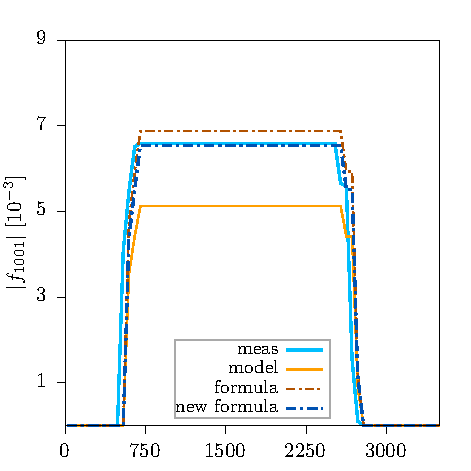
\includegraphics[width=.49\linewidth]{forcedcoupling/ac_outside_closed_bump}
  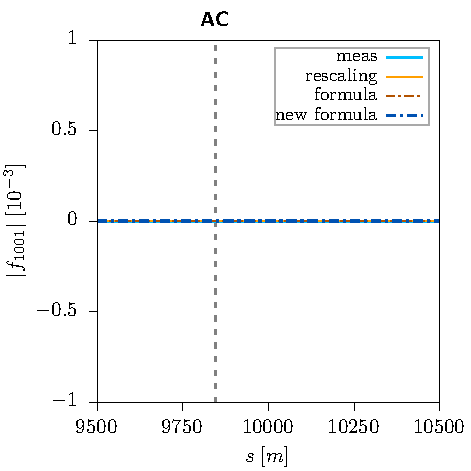
\includegraphics[width=.49\linewidth]{forcedcoupling/ac_outside_closed_bump_at_loc}
  \caption{Comparison of the three methods with a coupling bump in the lattice.
    The absolute value of coupling term $f_{1001}$ is shown.
    Formula method and new method (called \emph{new formula}) manage to reproduce well the $f_{1001}$.
    The naive rescaling method underestimates the $f$~term in the bump.
    The offset between \emph{meas} and the reconstructed values is due to the reconstruction
    of the complex signal.
    The right plot shows the region in which the AC-dipole is located.
    There is no jump at the location of the AC-dipole.
  }
  \label{fig_comp_felix_ryo_ac_outside}
\end{figure}
%
In Figure~\ref{fig_comp_felix_ryo_ac_outside} the case of a coupling bump in the lattice is shown.
The AC-dipole is located at $s=\SI{9846}{m}$ in a region with low coupling. As can be seen on the right plot
the jump at the location of the AC-dipole is non-existing. The formula method and the new method show a good
agreement with the measured values. The rescaling method underestimates the $f$~term inside the bump but outside
its accuracy is also excellent.
The measured values show an offset which is due to the reconstruction of the complex signal from the
momentum \eqref{eq_recon_AB} which picks up coupling sources from in between $s_a$ and $s_b$.
%
\begin{figure}[h]
  \centering
  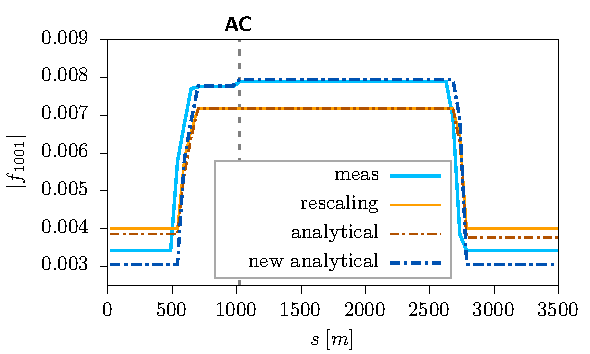
\includegraphics[width=.7\linewidth]{abs}
  \caption{Comparison of the three methods with the AC-dipole surrounded by a coupling bump.
    The AC-dipole is creating a jump in the coupling term $f_{1001}$ at its location. Only the new
    formula is able to reproduce this jump. The position of the AC-dipole is marked by a vertical
    line.
  }
  \label{fig_comp_felix_ryo}
\end{figure}
%

Figure~\ref{fig_comp_felix_ryo} now shows the picture when the AC-dipole is placed \emph{inside} the bump and,
thus, being in a region with strong coupling. In this case a visible bump is expected and the agreement with the
conventional methods should decrease because they do not consider the additional source.
Indeed, the new formula yields overall a better accuracy, especially inside of the coupling bump.
The jump at the position of the AC-dipole is well reproduced, as expected from \eqref{eq_drv_f1001_final}.

\section{Conclusion}

Current methods to calculated the coupling terms $f_{1001}$ and $f_{1010}$ in the LHC have been revised and
brought into context of recent findings. The AC-dipole creates a jump in the RDTs at its location and this jump
can be demonstrated for the coupling RDTs in simulations. A study of sextupolar RDTs is presented in~\cite{Carlier2020}.
The calculation of a corrected coupling RDT has been performed and its accuracy in the case of small coupling
has been demonstrated in simulations.